%!TEX encoding = UTF-8 Unicode
\chapter{Description of the Project}
\label{sec:Architecture}
%- Como pensam abordar a tese tendo em conta o problema, as contribuicoes a que propoe a dar e a arquitectura definida.
%- Descricao de alto nivel da arquitectura do sistema: Arquitectura do SW explicando os principais componentes e as funcoes que executam.
%- Como procederam as escolhas das ferramentas, linguagens de programcao, ambientes de desenvolvimento, hardware
%- Como prevem desenvolver a arquitectura proposta: por onde vao comecar. Como vao integrar os componentes, que dificuldades esperam encontrar e que estrategias planeam para as ultrapassar.
\noindent Based on the reviewed works, the solution proposed in this section is to develop and implement a novel architecture which will provide mobility support to fog nodes as well as to end devices in a simulation toolkit. Besides, it will also optimize the decision-making of migration by implementing multi-objective decisions into the algorithm, namely: QoS, cost, energy and bandwidth.
\section{Simulation Toolkit}
\noindent From Table \ref{tab:toolkits}, it can be clearly observed that most of the existing simulation toolkits are CloudSim-based. More recent works in fog computing have begun to implement their investigation works in iFogSim, which is also based on CloudSim. Moreover, recently some other simulators have been proposed as extensions to iFogSim. Since such attention has been given to this ``family'' of simulators, which count with a larger community, information and documentation compared to other isolated simulators, our work will be based on iFogSim.\\
\noindent\tab On the one hand, iFogSim already has really fortunate characteristics. For instance, it has built-in energy (based on CPU utilization), cost (depending on memory, storage, bandwidth and CPU utilization), application (by defining deadlines for modules and applications) and communication models (by defining delays and bandwidth). Also, it already supports virtualization techniques (using VMs). Moreover, this simulator supports DDF programming model, where different modules may be deployed in different machines, creating dependencies between them. In other words, an application module at a given machine is responsible for processing all data generated from modules hosted at machines below in the hierarchy. On the other hand, this simulator has some minor negative points compared with other simulators (refer to Table \ref{tab:toolkits}), however those are not critical. For example, the built-in communication model is unrealistic by disregarding low-level network issues such as link errors or congestion-related losses. However, these can be treated as high-level attributes such as latency or bandwidth of connections. Moreover, as berofe mentioned, GreenCloud is a more fine-grained simulator in what respects to energy consumption. Still, in iFogSim, energy models are able to vary according to the CPU usage. Furthermore, as network usage is already measured in both directions (downlink and uplink), it is possible to take into account those values in the calculation of energy consumption (as we intend to do).\\
\noindent\tab Despite the above-mentioned issues, iFogSim still has some major drawbacks such as not providing communication between fog nodes at the same level; rather it only provides parent-child communication. This feature is of most importance as discussed before (e.g., to implement an architecture based on fog colonies). Moreover, it does not allow mobility of fog nodes nor end devices and its application placement is static.%; does not consider any dynamic environment (although it already provides interfaces to ease this implementation).

\section{Data Placement Optimization}
\noindent Based on iFogSim, in order to achieve the desired objectives, firstly is necessary to implement ``horizontal'' communication between fog nodes.\\
\noindent\tab At the beginning of each simulation, iFogSim executes a placement strategy which is responsible to distribute the miscellany of application modules among the available fog nodes. These nodes are deployed in a hierarchical manner where each fog node has a parent (except for the cloud). Thus, a path is composed by the intermediate fog nodes, the links between them, the cloud and the gateway (fog node which is connected to the sensors and/or actuators). This strategy, favors the placement of modules closer to the end devices.
%%
%%
As already mentioned, modules have some dependencies (i.e. the data from one module may be the input of other module). Specifically, this strategy goes for each fog node in a given path search for what are the modules that can be placed (i.e. all their predecessors/dependencies were already placed in south fog nodes). Then, for each one of these modules, it will verify if the current node is able to host it, based on the available CPU. If not, the module is transferred vertically in the hierarchy until some machine is able to host it. This is poorly efficient in terms of load balancing, QoS guarantees and search complexity. It is worth noting that this strategy is performed before the actual simulation begin. Therefore it does not take into account the real migration problems.\\
\noindent\tab Our aim is to search not only vertically but also along all neighborhoods. In a first stage, as iFogSim does not considers geographical positioning of fog servers, we will assume that fog nodes at the same level, are in the close vicinity. Once this is achieved,
%our objective is to somehow divide the whole system. As aforementioned, this algorithm is not very efficient. It may work for systems composed by few fog nodes, but as the system grows to a bigger scale, it would not be feasible.
%Thus, 
in order to provide scalability, we aim to divide the search problem into small systems (e.g., as fog colonies does). To do so, we aim so implement graph partitioning functionality that iFogSimWithDataPlacement simulator has already implemented. Specifically this feature is implemented using three components. First, the graph modeling engine creates an undirected graph where vertices represent fog nodes and edges model physical links. Then, the graph weighting engine is responsible for allocate weights to both vertices (based on the number of data items produced in each fog node) and edges (based on the number of data flows passing through these links). Finally, the graph partition engine is responsible to apply a k-way partitioning method to divide it into $k$ sub-graphs using Metis \cite{METISSer49:online}, applying the typical criteria: balancing the vertex weights between sub-graphs and minimizing the sum of cut edges weights. We also intend to compare this approach with different criteria such as the end-to-end latency, physical distance or network distance (i.e. number of hops).\\
\noindent\tab At this point, we are now able to implement and test some algorithms proposed in the reviewed literature (refer to Section \ref{sec:Migration}) and described later. This would take into account the available parameters in iFogSim to minimize latencies and some other objectives such as energy, cost, bandwidth and, afterwards, jointly consider them all. To perform this implementation, iFogSim already has some built-in valuable attributes, as shown below:
\begin{multicols}{3}
		\begin{itemize}[noitemsep]
			\item costPerCPU
			\item costPerMem
			\item costPerStorage
			\item costPerBw
			\item uplinkLatency
			\item uplinkBandwidth
			\item downlinkBandwidth
			\item idlePower
			\item busyPower
	\end{itemize}
\end{multicols}
As such, it will be possible to model the minimization problems and solve them with the algorithms presented in Section \ref{sec:optalgorithms}. The objective is to evaluate their performance in terms of both actual optimization and computational complexity. Note that at this stage we are facing a static environment where the optimization is performed before the actual simulation.

\section{Mobility Support}
After the above implementation, the aim is to provide mobility support. For this purpose MyiFogSim, which is also an extension of iFogSim, already provide some important features. It provides mobility support to end devices through migration of virtual machines between fog nodes. On the one hand, their approach introduces the migration policy which is responsible to answer to \textit{when} the VM should be migrated using the user movement (i.e. position, speed, and direction). On the other hand, upon the decision to migrate, they have introduced the migration strategy which defines \textit{where} and \textit{how} the VM should it be migrated. While the former defines when the migration should happen in order to guarantee QoS in the process, the latter regards to the type of migration (i.e. non-live container/VM migration or VM live migration using post-copy) and simple strategies to define the fog node destination such as shortest distance or lowest latency. However, as some review works have shown (e.g., \cite{sun2016primal,zhang2016segue}), these greedy strategies are not perfect at all, and other parameters have to be taken into account. Hence, this work intends to implement some work already performed, but extend it to incorporate new features and exploit aspects that were not yet explored. Besides, this work also aims to provide fog servers mobility. %Afterwards, is also objective to adjust the previous optimization to take into account mobility patterns (e.g., as B. Ottenwälder et al. \cite{ottenwalder2013migcep} did).

\section{Architecture}
Based on the above mentioned our implementation consists in applying the architecture presented in Figure \ref{sw_architecture}. Grey classes are from iFogSim and CloudSim simulators, yellow classes are from MyiFogSim simulator and the green ones are from iFogSimWithDataPlacement. Note that those classes are the ones presented in the corresponding papers, being only the most important ones in their implementations. Our implementation will be focused in the white classes. It is worth mentioning that both MyiFogSim and iFogSimWithDataPlacement, as shown in Table \ref{tab:toolkits}, do not have documentation and some errors were already found.\\ %Therefore, it is high unpredictable to estimate the efforts that it will require to aggregate their implementations.
\noindent\tab As it can be seen, our work will implement four main classes, namely: MobileFogDevice, GA, PSO and MDP. The MobileFogDevice class will extend FogDevice. Therefore, it will inherit all its attributes and methods. Besides, it will have an object of MobileDevice from MyiFogSim, containing attributes such as the direction, speed and geographical position. The remaining classes will focus on implementing some optimization algorithms reviewed in Section \ref{sec:Migration}. Note that, at this moment is difficult to define \textit{when} the optimization algorithm recalculation will be performed. This is because, first we need to evaluate their behavior in terms of computational complexity and execution time. However, based on the reviewed literature, there are three options. The first, proposed by MyiFogSim, is to recalculate only when the user is predicted to go out of range from a base station. Based on its position, direction and speed it is possible to predict an handover. When this is verified, the algorithm is executed to compute the best placement to its VM (compute the cloudlet destination). Another approach is to recalculate periodically, but the optimal time interval is never specified (it is only said that it depends on the system dynamics). Finally, the third approach, is to only recalculate when a QoS violation is predicted. This would evolve several parameters such as server and network states as well as mobility and request patterns (e.g., as W. Zhang et al. \cite{zhang2016segue} and B. Ottenwälder et al. \cite{ottenwalder2013migcep} did).

\begin{figure}
	\centering
	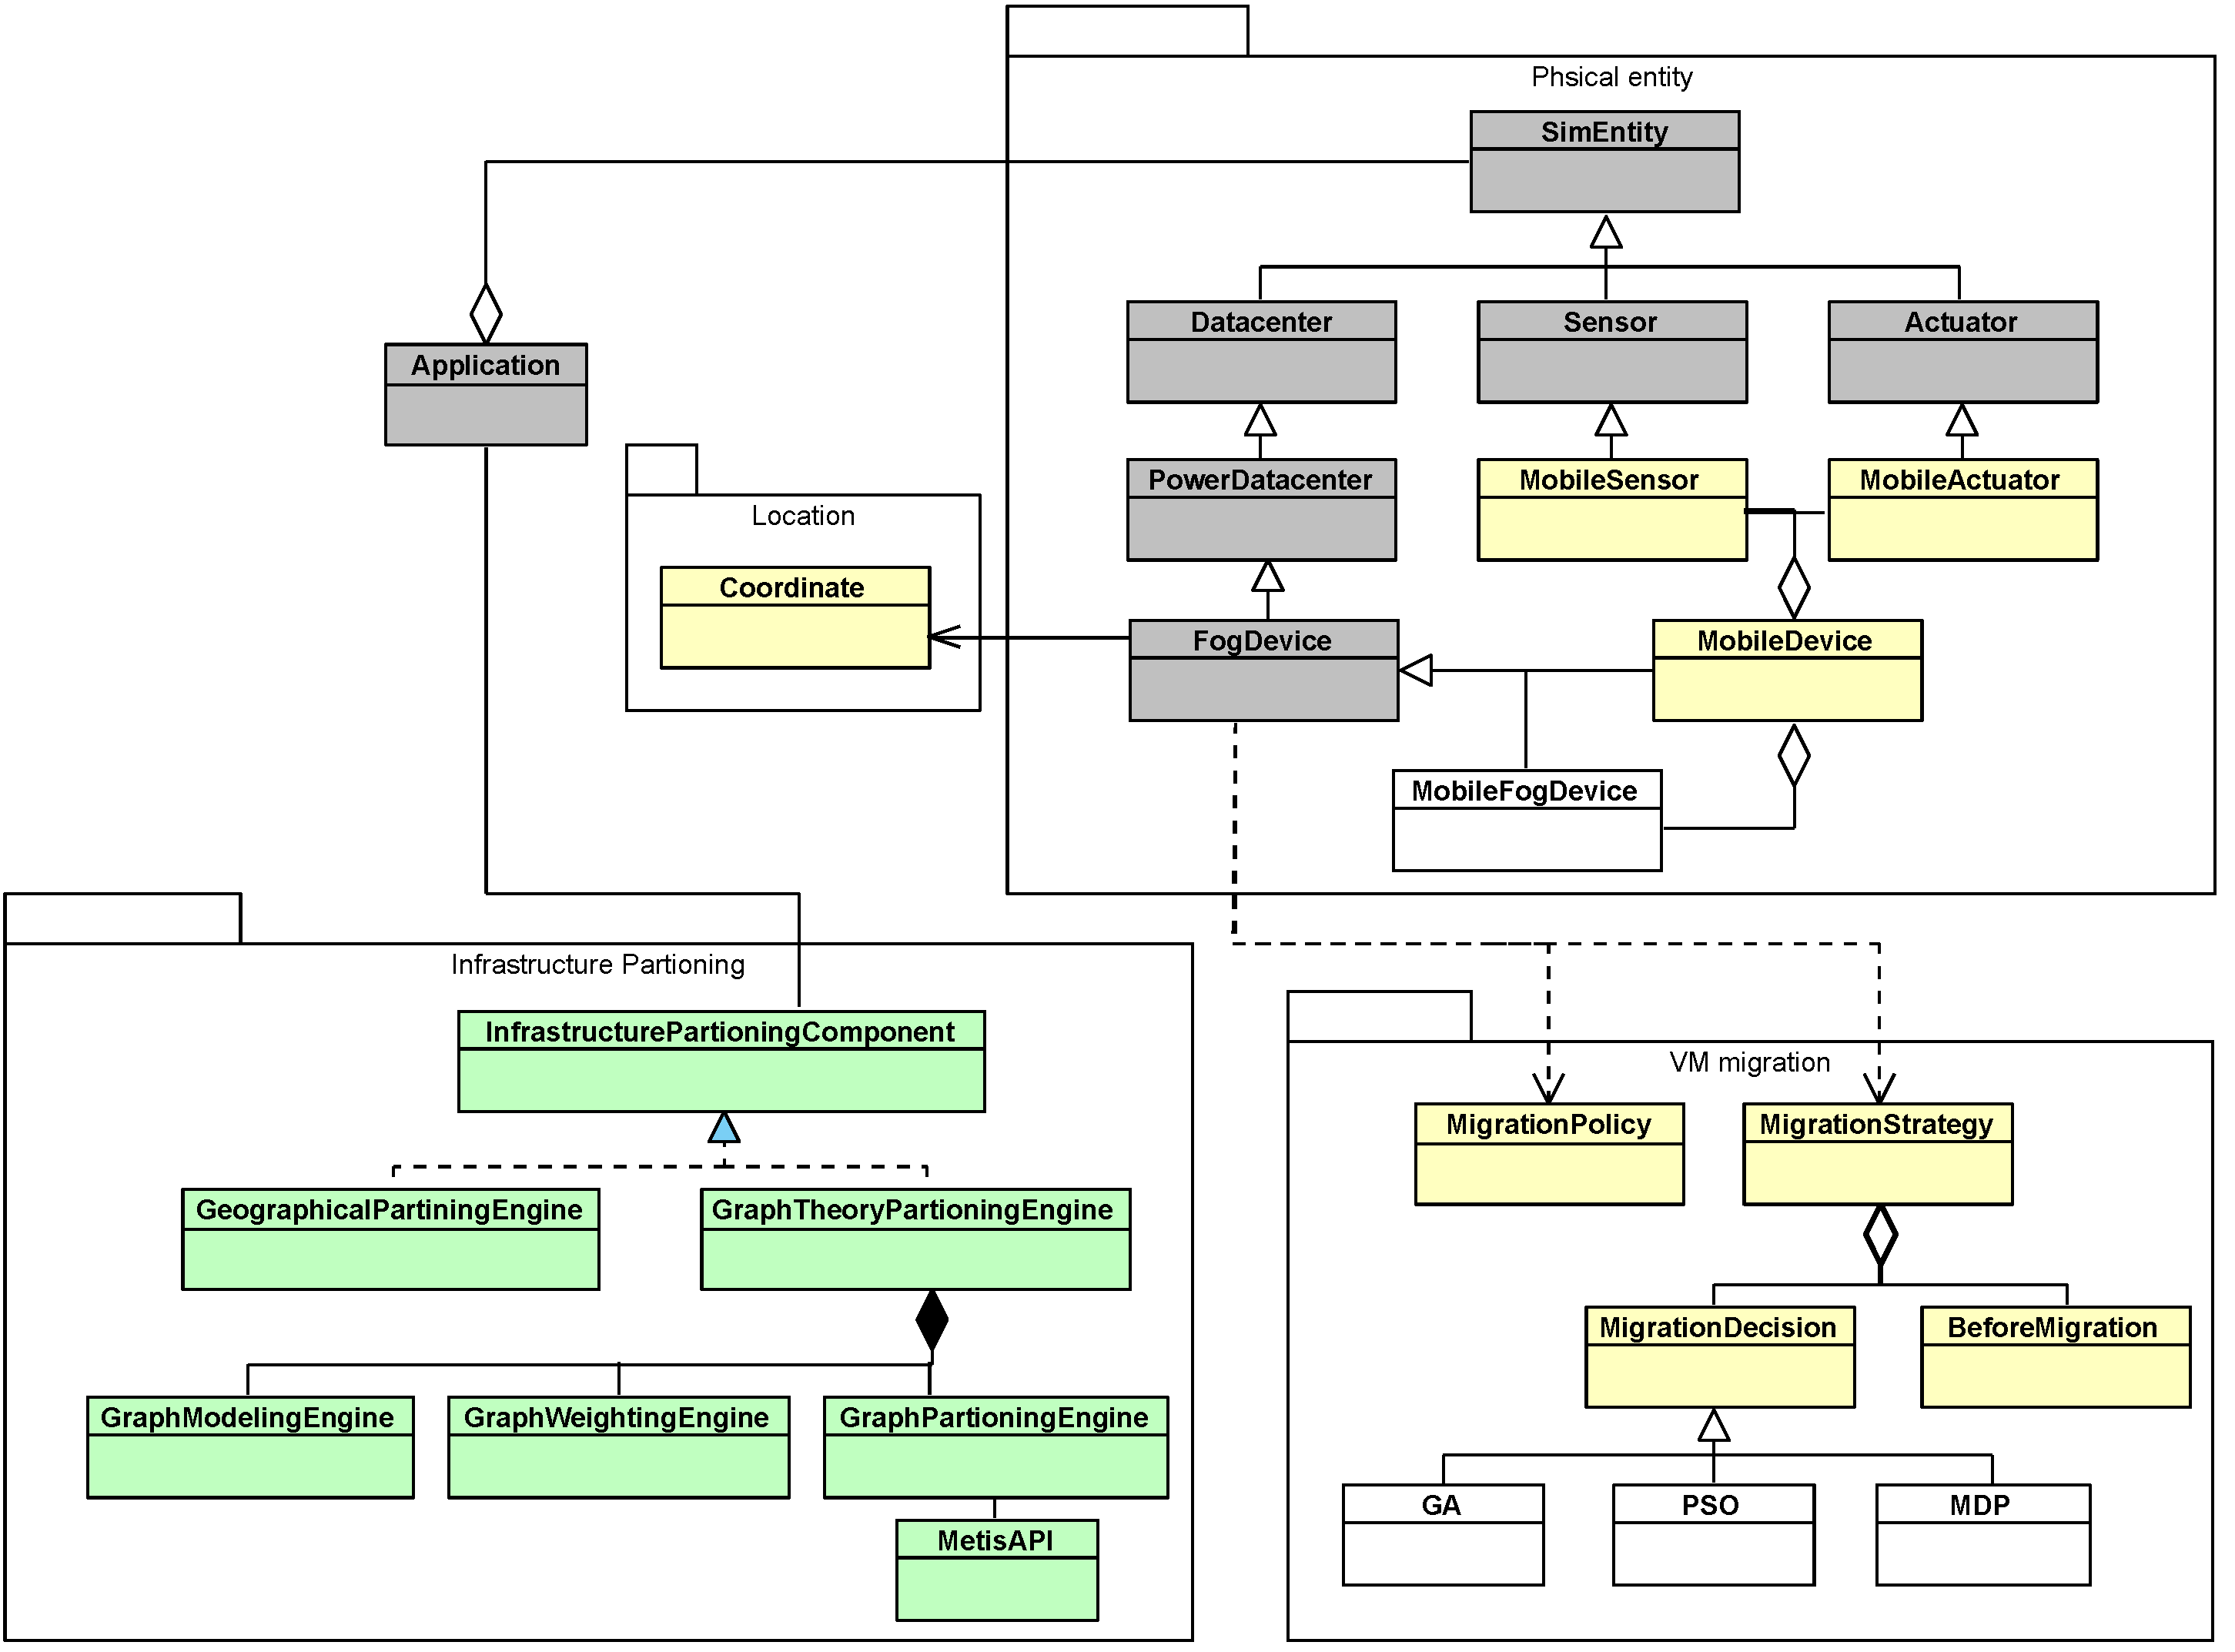
\includegraphics[width=0.9\textwidth]{images/sw_architecture/sw_architecture}
	\caption{UML Class diagram of the main added functionalities.}
	\label{sw_architecture}
\end{figure}

\section{Optimization Algoritms}\label{sec:optalgorithms}
As already mentioned, we intend to implement and test some proposed algorithms in the reviewed literature. From the panoply of solvers, we intend to study the behavior of the three presented below. Later, depending on the available time, more algorithms may be tested.

\subsection{Genetic Algorithm}
\noindent GA is an adaptive heuristic search algorithm. It is based on the idea of natural selection and genetics. Specifically, it is an iterative random search which is able to provide high-quality solutions for optimization problems and search problems.\\
\noindent\tab The algorithm has an arbitrary number of individuals composing the population. During the process, each iteration is characterized by a generation of individuals (of size population). Each individual represents a point in the search space and a possible solution. Yet, for each iteration, it is simulated the process of natural selection or ``survival of the fittest''. Each individual has a chromosome with genes. By evaluating them, it is possible to define its fitness score. Using this score, there are three operations in the creation of the next generation, namely: the selection operator which selects the individuals that will be part of the next generation, the crossover operator which represents mating between two individuals, resulting in a new individual with a chromosome composed by random genes from the two parents, and, finally, the mutation operator which will randomly introduce genes in the individuals resulting from the crossover operator to maintain the diversity in population to avoid the premature convergence \cite{whitley1994genetic}.

\subsection{Particle Swarm Optimization}
\noindent PSO is inspired by flocking behavior of birds and the schooling behavior of fish. PSO resembles the approach that bees take to find the right flower to collect honey from, or swarms of birds and how they behave collaboratively, as a super-organism. In this case, unlike GA, there is no creation or deletion of individuals. Instead, they move on a landscape where their fitness is measured over time.\\
\noindent\tab In this algorithm, particles are initialized with random solutions. Each particle will store the best fitness for itself and for the swarm as a whole. Each particle will identify the global best by comparing its best finding with all best findings of all particles. Then, they will compute the vector which will conduct them in the direction of the global best. The movement is characterized by the time step and velocity. Note that an initialization with spread of particles too local will possibly lead to a local minimum finding, while a too spread out, will possible not converge \cite{kennedy2011particle}.

\subsection{Markov Decision Process}
\noindent Unlike the previous ones, MDP belongs to the Reinforcement Learning (RL) family of Machine Learning (ML) algorithms. RL refers to goal-oriented algorithms where a software agent is supposed to determine the ideal behavior within a specific context in order to maximize its performance (i.e. some notion of cumulative reward). So that the agent learn its behavior, a reward feedback is required (i.e. reinforcement signal). When this process is repeated, it is known as a Markov Decision Process.\\
\noindent\tab In this model, there are a set of possible states where the agent can be in, a set of models, a set of possible actions, a real valued reward function and a policy. A model or transition model defines the probability to go to state $s'$, while being at state $s$ and taking action $a$. The real valued reward function or, simply, reward indicates the benefit to take action $a$ while being at state $s$ and ending up in state $s'$. The policy, which represents the goal, is responsible to give the optimal action to take in every state. Finally, in order to solve MPDs it is needed to resort to dynamic programming (a method which divides the whole problem into smaller and simpler sub-problems), more specifically the Bellman equation \cite{bellman1957markovian,bertsekas2005dynamic}.


%A arquitetura dos Bus é boa (APs com várias cloudlets etc....)

%Starting from available simulators a significant programming effort is required to obtain a simulation tool meeting the actual needs.
%Simply applying existing radio access-oriented MM (mobility management) schemes leads to poor performance mainly due to the co-provisioning of radio access and computing services of the MEC-enabled (mobile edge computing) BSs (base stations).
%On a self-driving vehicle, are estimated to generate about 1GB data per second \cite{angelica2013google}. As the number of features grow, the data deluge grows out of control. Moreover, these types of systems, where people's lives depends on it, are hard real-time what means that it is absolutely imperative that all deadlines are met. Offloading tasks to fog nodes will be the best solution, once a big effort in mobility support has been  through the migration of VMs using cloudlets \cite{lopes2017myifogsim}. Also, in this context, Puliafito et al. address three types of applications where fog is required, namely, citizen's healthcare, drones for smart urban surveillance and tourists as time travellers \cite{puliafito2017fog}, addressing the needs of low latency and mobility support.\\